% Creating the chapter for Sprint 3
\chapter{Sprint 3 : Système d'alertes et de notifications}
\label{chap:sprint3}

% Introducing the chapter
\section*{Introduction}
\addcontentsline{toc}{section}{Introduction}
Le troisième sprint du projet VitalSync s’appuie sur le pipeline de traitement des données établi lors du sprint précédent, en se concentrant sur le développement des fonctionnalités essentielles pour la génération d’alertes, la distribution des notifications et l’interaction avec le personnel médical. Ces fonctionnalités sont cruciales pour atteindre l’objectif du système, qui est de surveiller les signes vitaux en temps réel et de permettre une réponse rapide dans un contexte médical. Ce chapitre détaille les objectifs du sprint, les activités réalisées, les livrables produits, les tests effectués, les défis rencontrés, la rétrospective de l’équipe et la planification pour le sprint suivant. Des diagrammes UML sont intégrés pour illustrer la conception et le flux de travail du système, renforçant la compréhension des interactions entre les composants.

% Describing the objectives
\section{Objectifs}
L’objectif principal du sprint 3 était d’enrichir le système VitalSync avec des fonctionnalités clés pour la surveillance en temps réel et la réactivité face aux anomalies. L’équipe a cherché à implémenter un mécanisme d’évaluation des règles d’alerte permettant de détecter les anomalies dans les signes vitaux, en s’appuyant sur des seuils spécifiques à chaque patient stockés dans une base de données. Lorsqu’une anomalie est détectée, le système génère et enregistre une alerte associée aux données du patient. Les alertes critiques déclenchent des notifications envoyées au personnel médical via Firebase Cloud Messaging (FCM). Une interface préliminaire, développée avec Laravel pour le backend et React pour le frontend, a été conçue pour permettre au personnel médical de visualiser les alertes, d’accéder aux données des patients et de confirmer la réception des notifications. L’API Flask a été étendue pour intégrer la logique des alertes et des notifications, posant ainsi les bases pour des améliorations futures de l’interface utilisateur.

% Detailing the tasks
\section{Activités}
Le sprint 3, d’une durée de trois semaines, s’est articulé autour d’activités clés visant à faire progresser les fonctionnalités du système. Une première activité a consisté à développer un système d’évaluation des règles d’alerte. Ce système analyse les données des signes vitaux, telles que la fréquence cardiaque ou la pression artérielle, en les comparant aux seuils spécifiques stockés dans la base de données MySQL. L’API Flask a été adaptée pour interroger ces seuils et effectuer les comparaisons nécessaires, assurant une détection précise des anomalies. Une fois une anomalie détectée, le système génère une alerte liée au dossier du patient, enregistrée dans la base de données avec des attributs tels que la priorité et l’état (par exemple, active ou confirmée). Cette approche garantit une traçabilité fiable des alertes et prévient toute perte de données.

Pour la distribution des notifications, un système basé sur Firebase Cloud Messaging a été implémenté afin d’envoyer les alertes critiques aux appareils mobiles du personnel médical, identifiés via leurs rôles dans la base de données. Cette intégration permet une communication rapide et ciblée, essentielle pour répondre aux situations urgentes. Une interface préliminaire, développée avec Laravel et React, a été mise en place pour permettre au personnel médical de visualiser les alertes, d’accéder aux données des signes vitaux et de confirmer la réception des notifications. Ces confirmations mettent à jour l’état des alertes dans la base de données, assurant une traçabilité complète. Les préférences des utilisateurs, telles que les paramètres de notification, ont également été enregistrées pour personnaliser l’expérience.

L’API Flask a été optimisée pour gérer la logique des alertes et des notifications, en s’intégrant harmonieusement avec le backend Laravel. Cette intégration permet une communication fluide entre les composants du système, tandis que l’interface préliminaire offre des fonctionnalités de filtrage de base pour les données des patients et les alertes. Ces développements préparent le terrain pour des améliorations futures, notamment en termes de visualisation et d’ergonomie, prévues pour le sprint suivant.

% Illustrating the workflow with UML diagrams
\subsection*{Diagrammes d'illustreration du flux de travail}
Pour illustrer le flux de travail des alertes et des notifications, plusieurs diagrammes UML sont proposés en complément du diagramme de classes déjà présent. Le diagramme de séquence, présenté dans la figure~\ref{fig:sprint3_sequence_diagram}, décrit les interactions entre les composants du système, depuis le traitement des données des signes vitaux jusqu’à la livraison des notifications et leur confirmation par le personnel médical. Ce diagramme met en évidence la séquence des appels entre l’API Flask, le backend Laravel, Firebase Cloud Messaging et l’application mobile Flutter, offrant une vue claire du flux de données.

\begin{figure}[H]
    \centering
    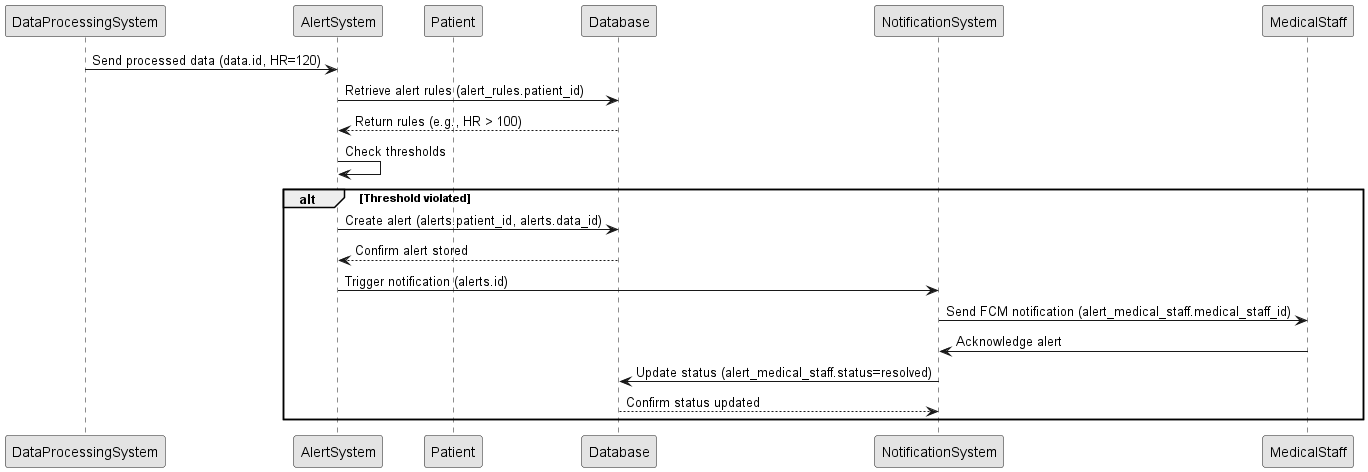
\includegraphics[width=0.8\textwidth]{chapter6/diagrams/sprint_sequence_diagram.png}
    \caption{Diagramme de séquence pour la génération d'alertes et la distribution des notifications}
    \label{fig:sprint3_sequence_diagram}
\end{figure}

Un diagramme d’activité est également recommandé pour compléter l’analyse. Ce diagramme illustrerait le processus global de gestion des alertes, depuis la réception des données des signes vitaux jusqu’à la confirmation des notifications par le personnel médical. Il mettrait en lumière les décisions prises, comme la comparaison des données avec les seuils, et les flux parallèles, tels que l’envoi simultané de notifications push via FCM et d’e-mails via le backend Laravel. Ce diagramme d’activité offrirait une perspective complémentaire en détaillant les étapes du processus et les points de décision, renforçant la compréhension des interactions dynamiques (voir Figure~\ref{fig:sprint3_activity_diagram}).

\begin{figure}[H]
    \centering
    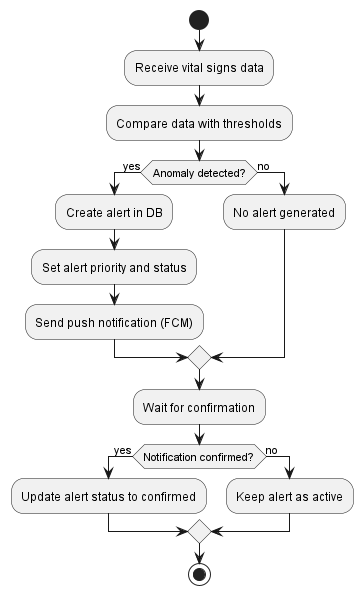
\includegraphics[width=0.9\textwidth]{chapter6/diagrams/sprint_activity_diagram.png}
    \caption{Diagramme d'activité pour le processus de gestion des alertes}
    \label{fig:sprint3_activity_diagram}
\end{figure}

Enfin, un diagramme de cas d’utilisation spécifique à ce sprint est proposé pour représenter les interactions des acteurs, tels que les médecins et les infirmiers, avec le système, notamment pour la visualisation des alertes, la réception des notifications et la confirmation des actions. Ce diagramme complète le diagramme global des cas d’utilisation en se concentrant sur les fonctionnalités spécifiques du sprint 3, telles que la gestion des alertes et la personnalisation des notifications (voir Figure~\ref{fig:sprint3_use_case_diagram}).

\begin{figure}[H]
    \centering
    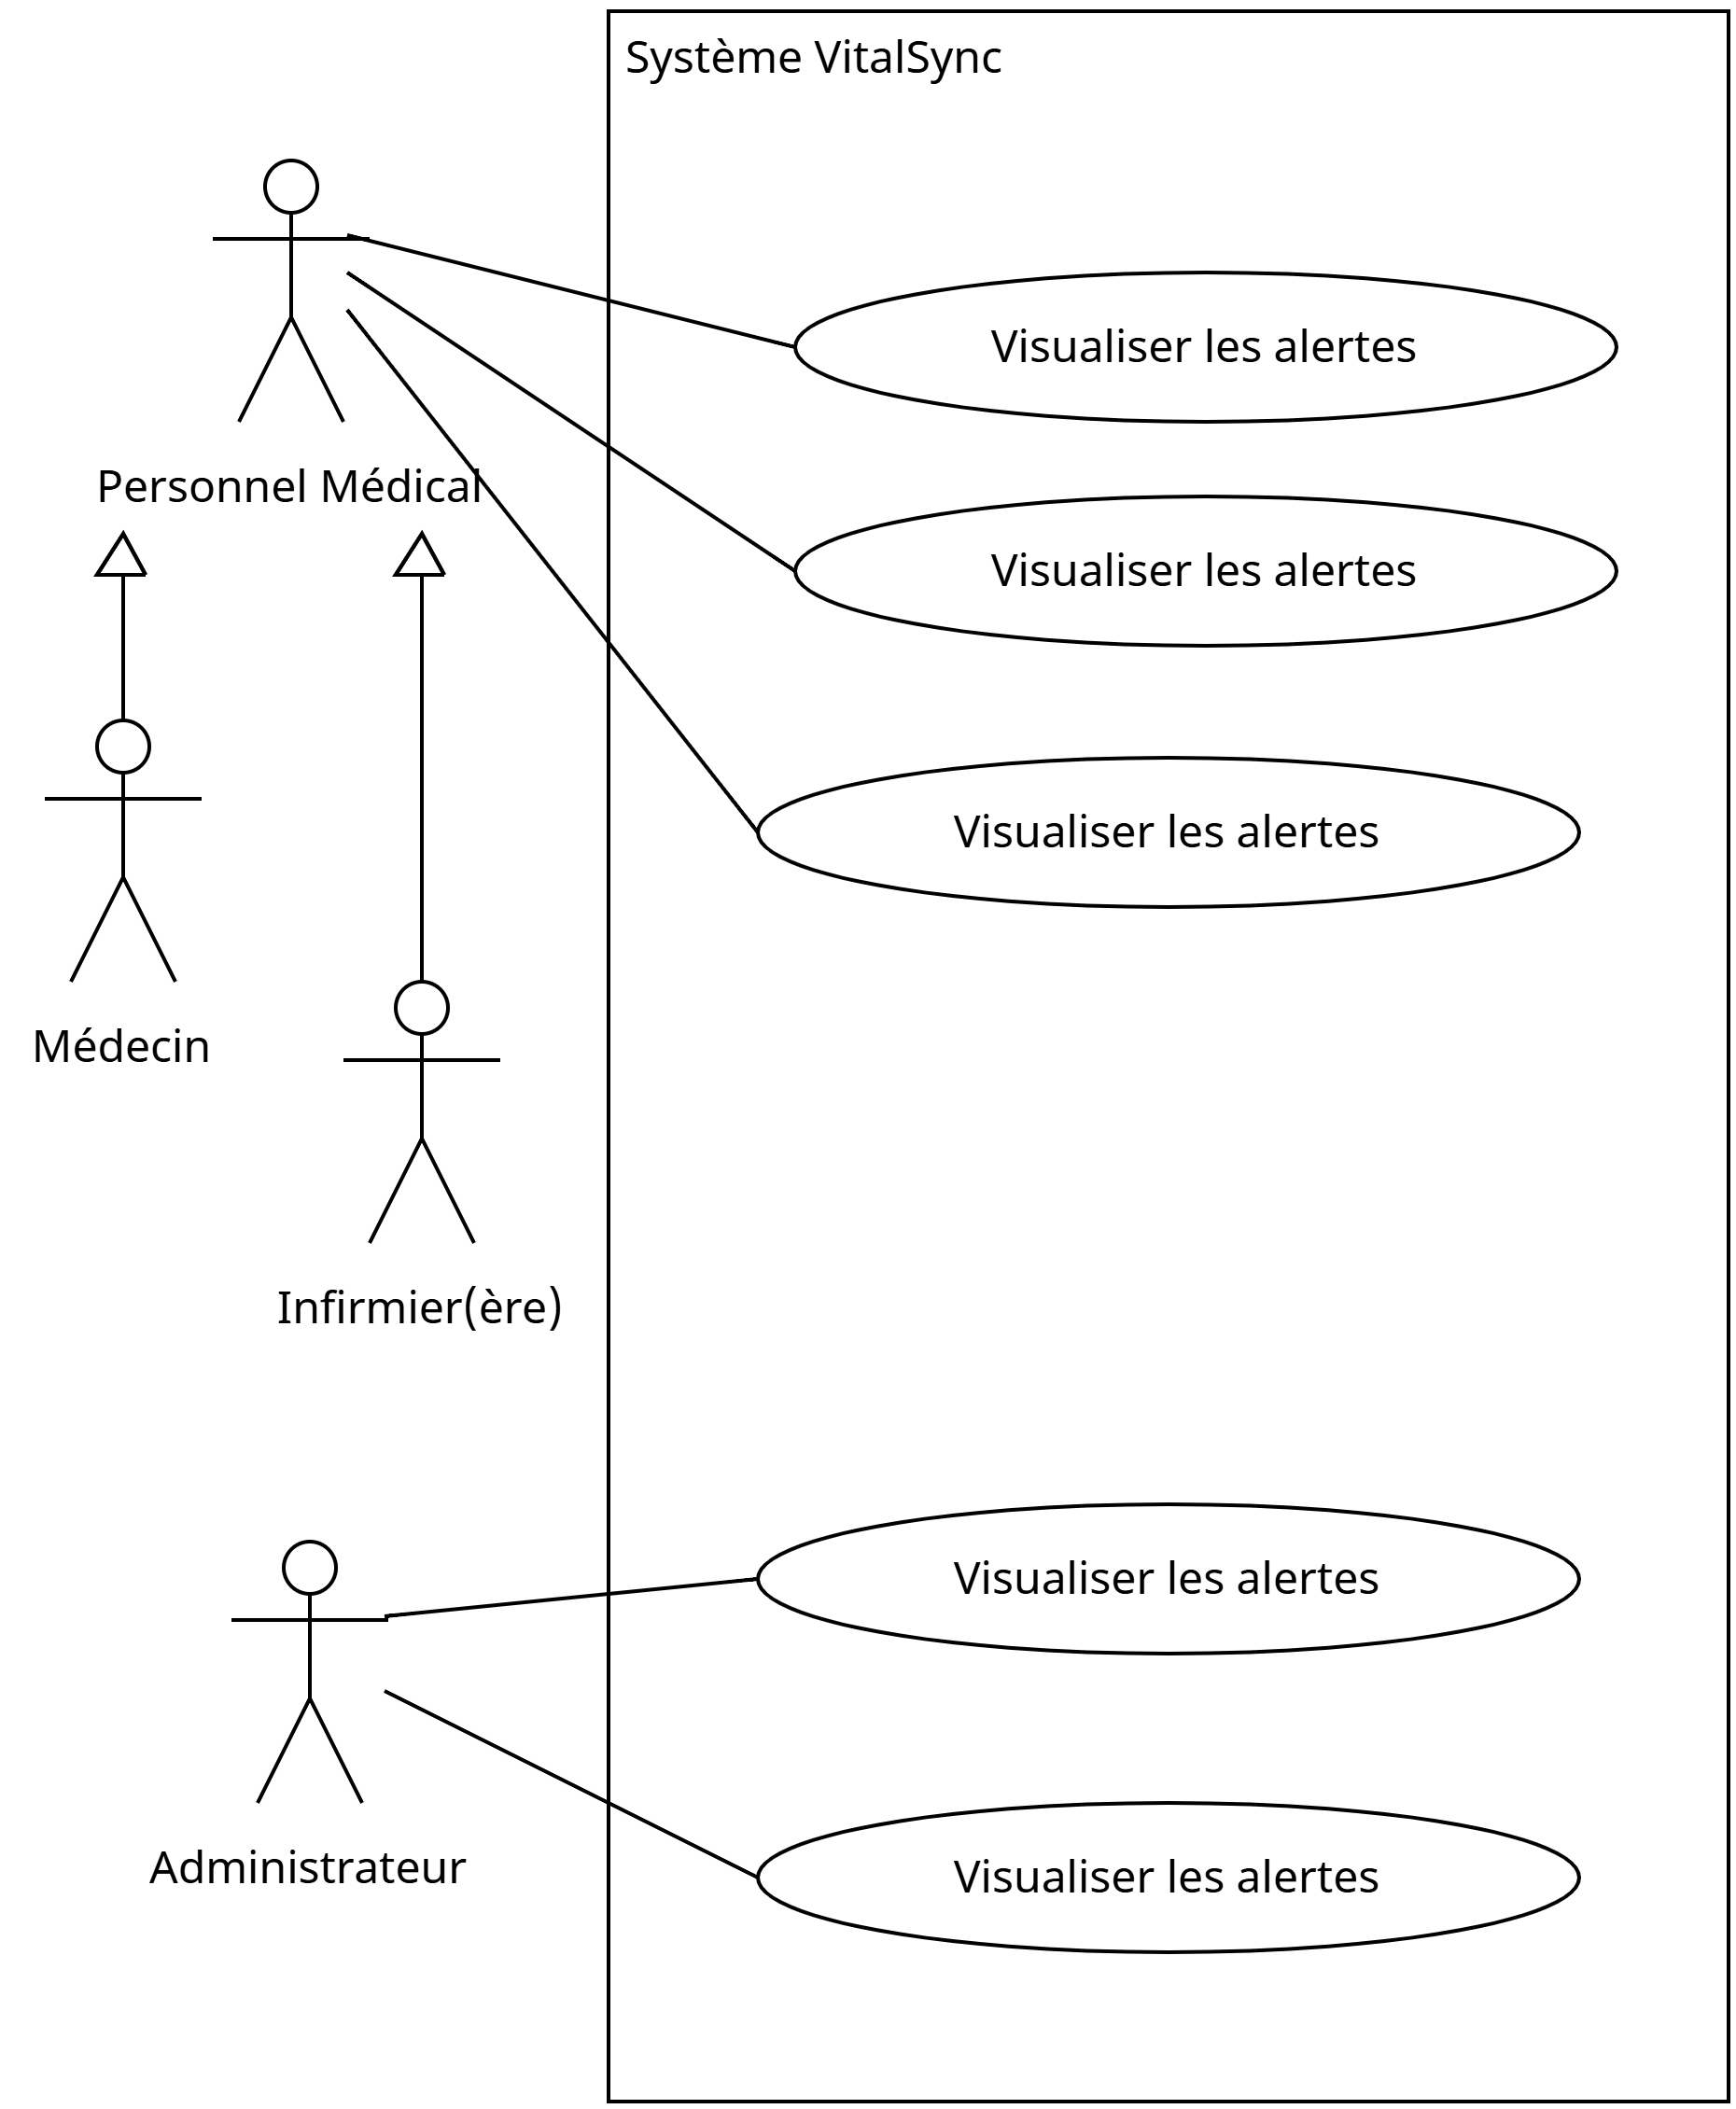
\includegraphics[width=0.8\textwidth]{chapter6/diagrams/sprint_use_case_diagram.png}
    \caption{Diagramme des cas d'utilisation pour le sprint 3}
    \label{fig:sprint3_use_case_diagram}
\end{figure}

% Listing the deliverables
\section{Résultats}
Le sprint 3 a permis de livrer plusieurs composants essentiels pour le système VitalSync. Un système d’alertes intégré à l’API Flask a été développé, capable de détecter les anomalies en fonction des seuils définis. Un système de notifications basé sur Firebase Cloud Messaging a été mis en place pour assurer une livraison rapide des alertes critiques au personnel médical. Une interface préliminaire, construite avec Laravel et React, permet la visualisation et la gestion des alertes, ainsi que l’accès aux données des patients. Le schéma de la base de données a été mis à jour pour inclure des tables dédiées aux alertes, aux notifications et aux préférences des utilisateurs, garantissant une gestion efficace des données. Une documentation complète, couvrant les points d’API, l’utilisation de l’interface et la configuration du système, a également été produite pour faciliter les développements futurs.

% Describing the testing process
\section{Tests}
Les tests ont validé les livrables du sprint 3 en évaluant plusieurs aspects du système. La précision du système d’alertes a été testée à l’aide de données simulées, démontrant une capacité fiable à détecter les anomalies des signes vitaux. La latence des notifications a été mesurée pour s’assurer qu’elle répondait aux exigences de temps réel, avec des résultats satisfaisants dans des environnements de test. La fonctionnalité de confirmation des alertes a été validée, confirmant que les mises à jour de l’état des alertes dans la base de données étaient fiables. Des tests d’intégration de bout en bout ont vérifié le flux de données, depuis la capture des signes vitaux jusqu’à la livraison des notifications, sans détecter d’erreurs critiques. Les résultats des tests ont été consignés pour servir de base à la rétrospective.

% Discussing challenges
\section{Défis}
Plusieurs défis ont émergé au cours du sprint 3. La configuration initiale de Firebase Cloud Messaging a rencontré des problèmes, entraînant des échecs intermittents dans la livraison des notifications. Ces problèmes ont été résolus en optimisant le middleware Laravel et en mettant à jour les identifiants FCM. Certaines alertes critiques présentaient une latence supérieure aux attentes, ce qui a nécessité une indexation des requêtes de la base de données et une mise en cache des seuils pour améliorer les performances. Enfin, le personnel médical a exprimé le besoin de fonctionnalités de filtrage avancées dans l’interface, une demande qui a été reportée au sprint suivant en raison des contraintes de temps.

% Summarizing the retrospective
\section{Rétrospective}
La rétrospective du sprint 3 a mis en évidence les succès et les points à améliorer. L’équipe a livré avec succès un système fonctionnel d’alertes et de notifications, répondant aux objectifs de surveillance en temps réel. Cependant, la sous-estimation du temps nécessaire à l’intégration de FCM a conduit à des ajustements dans la planification. Les réunions quotidiennes ont été affinées pour prioriser la résolution rapide des obstacles, ce qui a amélioré l’efficacité de l’équipe. La collaboration entre les équipes backend et frontend s’est renforcée, mais une fréquence accrue des sessions de retour avec le personnel médical a été recommandée pour mieux aligner le système sur les besoins des utilisateurs.

% Outlining Sprint 4 planning
\section{Planification pour le sprint 4}
Le sprint 4, prévu pour une durée de trois semaines, se concentrera sur l’optimisation du système et l’amélioration de l’expérience utilisateur. Les objectifs principaux incluent la réduction de la latence des notifications à un niveau encore plus bas, l’enrichissement de l’interface avec des fonctionnalités avancées de filtrage et des visualisations des tendances des signes vitaux, ainsi que la réalisation de tests d’acceptation avec le personnel médical pour valider l’utilisabilité. La documentation sera finalisée, et les préparatifs pour le déploiement commenceront, en mettant l’accent sur les retours des utilisateurs et les métriques de performance.

% Concluding the chapter
\section*{Conclusion}
\addcontentsline{toc}{section}{Conclusion}
Le sprint 3 a marqué une avancée significative pour le système VitalSync en mettant en place des fonctionnalités robustes d’alertes et de notifications. Les livrables, incluant un système d’alertes précis, une distribution rapide des notifications et une interface préliminaire, s’alignent sur l’objectif du projet de surveillance en temps réel. Les défis, tels que la configuration de FCM et l’ergonomie de l’interface, ont été surmontés, orientant le sprint 4 vers une optimisation des performances et une préparation au déploiement.